% !TEX root = ../main.tex
\section{Results}

\subsection{In-Sample Fit}
\begin{figure}[htbp]
\centering
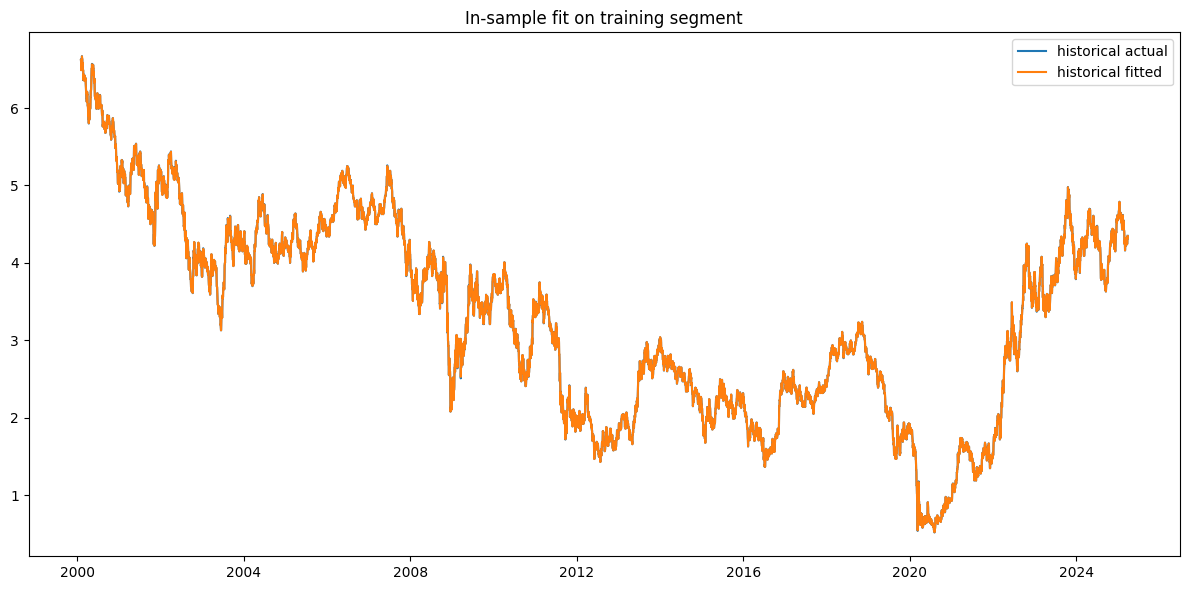
\includegraphics[width=\linewidth]{figures/insamplefit.png}
\caption{In-sample reconstruction of DGS10.}
\label{fig:insample}
\end{figure}
The model reconstructs the historical series with negligible error (RMSE $= 2.3\!\times\!10^{-3}$ on the level scale, MAPE $= 0.06\%$), indicating that the spectral representation is sufficiently expressive to capture both low-frequency trend behavior and higher-frequency oscillatory structure. Importantly, this fit is achieved through spectral synthesis rather than direct regression, implying that the learned amplitudes and frequencies form a complete functional basis for the observed signal.
The absence of visible lag or smoothing artifacts suggests that the phase dynamics are correctly learned, and that instantaneous frequency estimates are consistent with the underlying temporal structure. This supports the interpretation that the latent state encodes a dynamically evolving spectral representation rather than a static approximation.

\subsection{Conditional One-Step Forecast}
\begin{figure}[htbp]
\centering
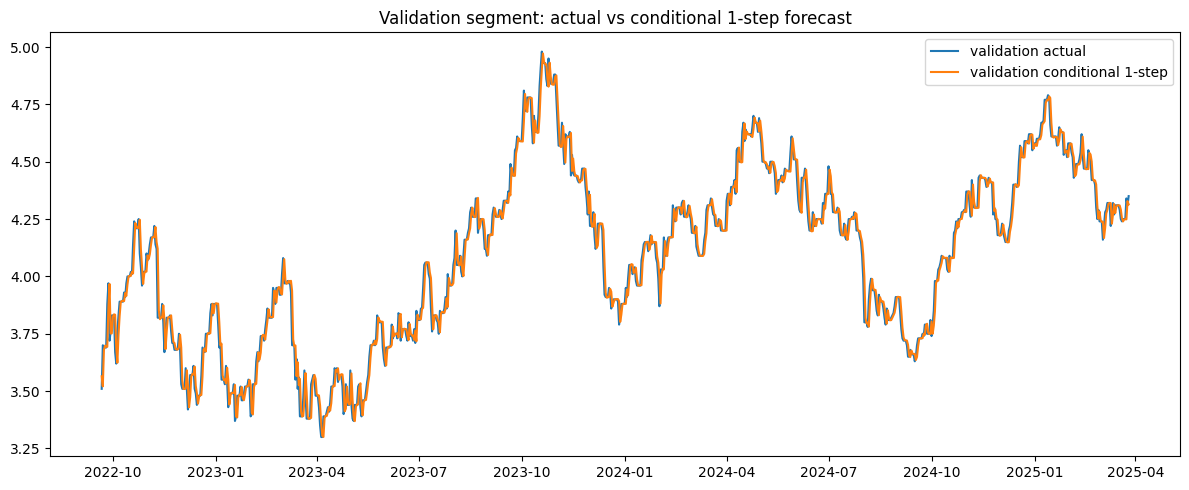
\includegraphics[width=\linewidth]{figures/validationsegmentactualvsconditional.png}
\caption{Conditional one-step forecast on holdout segment.}
\label{fig:forecast}
\end{figure}
The conditional one-step forecast closely tracks the realized series across the holdout period, with deviations confined to local fluctuations (holdout RMSE $= 3.87\!\times\!10^{-2}$, MAE $= 2.59\!\times\!10^{-2}$, MAPE $= 0.61\%$ on the level scale; RMSE $= 9.1\!\times\!10^{-3}$ on the log-yield scale). Because predictions are conditioned on observed data, this result isolates the representational capacity of the model from recursive error accumulation.
The alignment between predicted and observed values indicates that the latent state $h_t$ captures sufficient information to reconstruct short-term dynamics, including both trend adjustments and cyclical variation. In this regime, emission heads produce stable amplitude and frequency estimates, suggesting that the learned spectral parameters are locally consistent with the true data-generating process.

\subsection{Trend Component}
\begin{figure}[htbp]
\centering
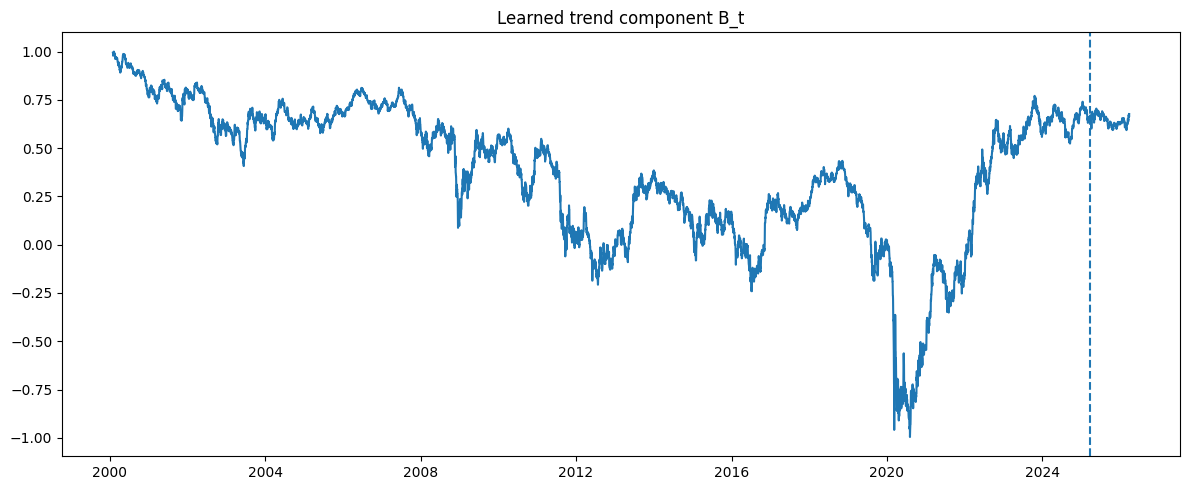
\includegraphics[width=\linewidth]{figures/learnedtrendb_t.png}
\caption{Learned trend component $B(t)$.}
\label{fig:trend}
\end{figure}
The learned trend component $B(t)$ captures the low-frequency structure of the DGS10 series, including the secular decline in yields over the sample period and the pronounced deviation associated with the 2020 shock. This separation indicates that the model isolates long-run movements from oscillatory components.
With smoothness regularization applied to $A_{t,k}$ and $\omega_{t,k}$, the trend head tends to absorb the low-frequency component while oscillatory terms capture higher-frequency variation. This separation is encouraged rather than architecturally enforced: in principle, slowly-varying amplitudes could also absorb low-frequency content. The empirically clean separation observed here therefore reflects the combined effect of the smoothness penalties and the inductive bias of the emission heads.

\subsection{Amplitude Dynamics}
\begin{figure}[htbp]
\centering
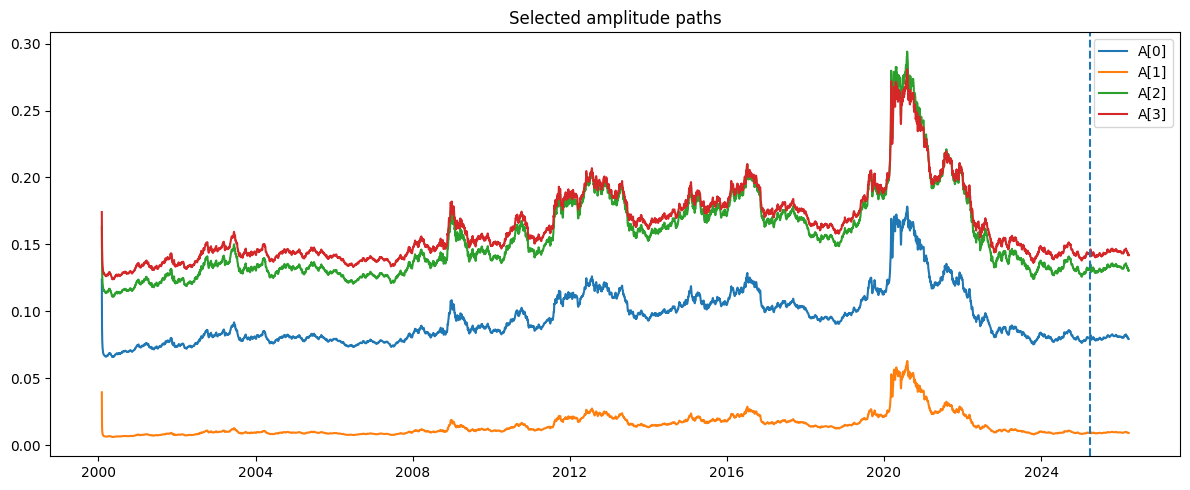
\includegraphics[width=\linewidth]{figures/selectedamplitudepaths.png}
\caption{Selected amplitude paths (four of $K=16$ components).}
\label{fig:amplitude}
\end{figure}
Amplitude paths $A_{t,k}$ serve as time-varying weights over spectral components and provide a direct measure of the relative importance of each oscillatory mode. The paths shown reflect the effective amplitudes after gate modulation. Several patterns emerge from the learned amplitudes.
First, there is a clear hierarchy across components, with a subset of amplitudes consistently dominating, indicating that the model concentrates explanatory power in a limited number of spectral modes. Second, during the 2020 regime shift, multiple amplitudes increase simultaneously, reflecting a temporary expansion in spectral complexity. This suggests that the underlying signal requires a richer combination of oscillatory components during periods of heightened macroeconomic uncertainty.
Following this period, amplitudes contract and stabilize, indicating a reduction in effective dimensionality. This behavior can be interpreted as adaptive spectral compression, where the model reduces the number of active components as the system transitions back to a more stable regime.

\subsection{Frequency Dynamics}
\begin{figure}[htbp]
\centering
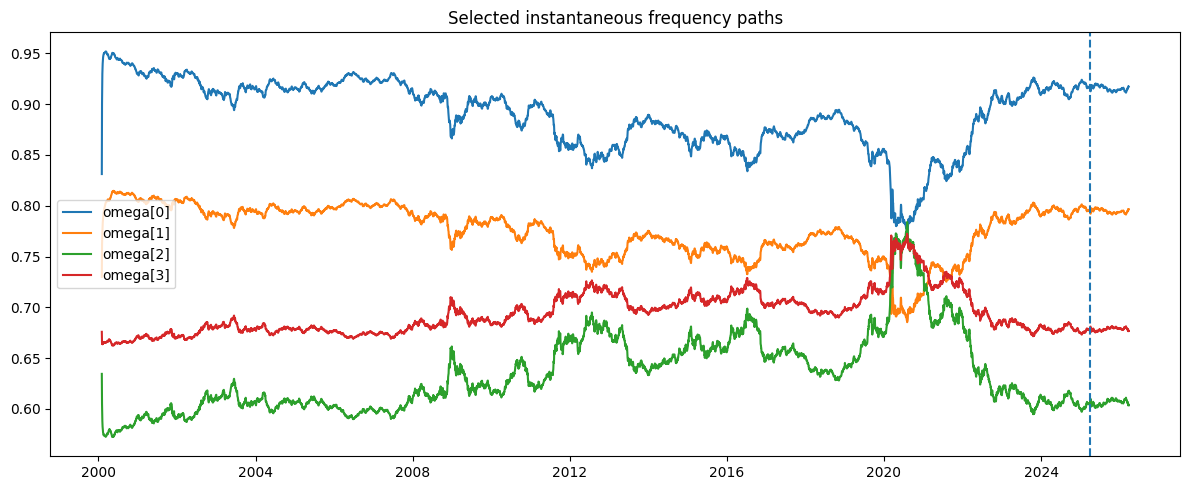
\includegraphics[width=\linewidth]{figures/selectedfrequencypaths.png}
\caption{Instantaneous frequency paths.}
\label{fig:frequency}
\end{figure}
Instantaneous frequency paths $\omega_{t,k}$ exhibit gradual drift over time under stable conditions, reflecting slow changes in cyclical structure. However, an apparent convergence of frequencies occurs during the 2020 period:
\begin{equation}
\omega_1(t) \approx \omega_2(t) \approx \cdots
\end{equation}
This convergence suggests that multiple spectral components align toward a common frequency, effectively reducing the dimensionality of the spectral representation. In functional terms, the decomposition appears to transition from a sum of distinct oscillatory modes to a smaller set of coherent cycles.
This phenomenon can be interpreted as a regime-dependent reduction in spectral diversity, where macroeconomic shocks compress the range of active frequencies. The ability of the model to represent this transition through learned emission heads provides qualitative evidence that instantaneous frequency carries meaningful structural information.

\subsection{Gating Behavior}
\begin{figure}[htbp]
\centering
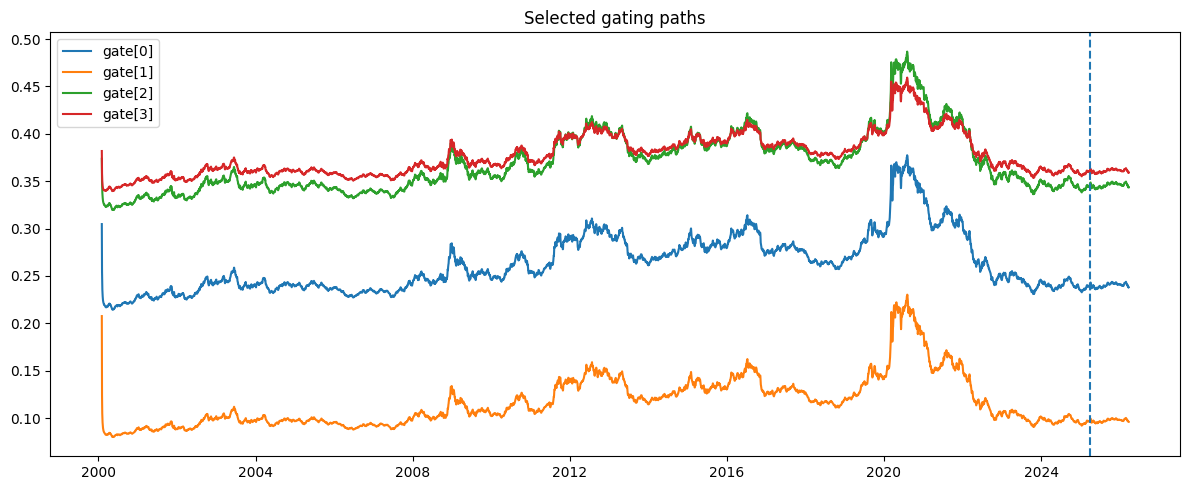
\includegraphics[width=\linewidth]{figures/selectedgatingpaths.png}
\caption{Gating weights $g_{t,k}$ across components.}
\label{fig:gating}
\end{figure}
Gating weights $g_{t,k}$ enter the synthesis ~\eqref{eq:synthesis} as multiplicative factors on each component, implementing the selection mechanism that determines which oscillatory modes are actively utilized at each time step. Unlike amplitudes, which control magnitude, gating values lie in $(0,1)$ and modulate component participation.
The learned gating paths exhibit persistent dominance of a subset of components, with others remaining suppressed throughout the sample. During the 2020 regime shift, gating weights increase for multiple components, consistent with the temporary expansion in spectral complexity observed in the amplitude paths.
After the shock, gating consolidates toward fewer dominant components, reinforcing the interpretation of adaptive model-order reduction. Together, amplitudes and gating weights implement a soft selection mechanism that allows the model to dynamically adjust the effective number of active spectral components in response to changing economic conditions.
